 \documentclass{report}
 
\usepackage[utf8]{inputenc} 
\usepackage[T1]{fontenc}      
\usepackage[top=2.0cm, bottom=3cm, left=3.0cm, right=3.0cm]{geometry}
\usepackage{graphicx}
\usepackage{wrapfig}
\usepackage{amsmath,esint }
\usepackage{amssymb}
\graphicspath{{figures/}{../figures}}

\newcommand*\dif{\mathop{}\!\mathrm{d}}
\newcommand*\diver{\mathop{}\!\mathrm{div}}
\newcommand*\grad{\mathop{}\!\mathrm{grad}}

\begin{document}

\section*{Induction mutuelle entre deux circuits}

On considère les deux circuits $LC$ suivants, composés de capacités $C_1$ et $C_2$ et de bobines d'inductance propre $L_1$ et $L_2$ et d'inductance mutuelle $M$. 

\begin{figure}[h!]
\centering
		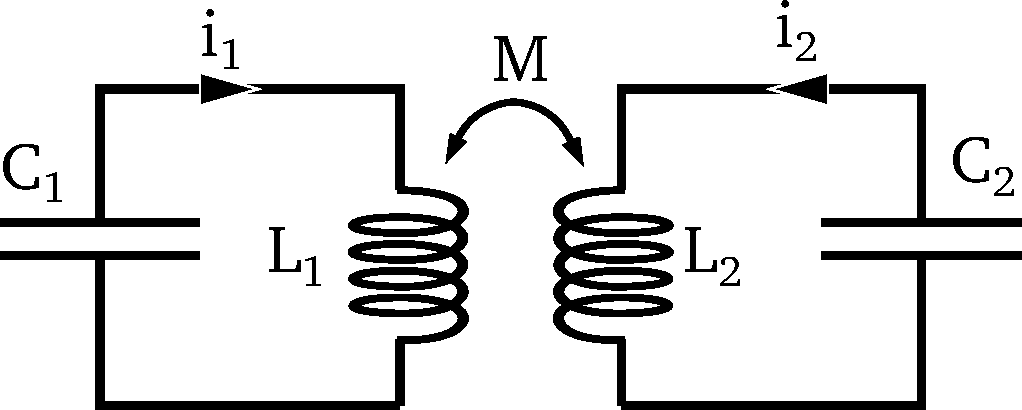
\includegraphics[scale=0.45]{induction_mutuelle.pdf}
\end{figure}

\begin{itemize}
	
	\item[$\clubsuit$] Qu'est-ce que l'inductance propre ? Leur induction mutuelle ? Quelle condition a t-on nécessairement entre $L_1$, $L_2$ et $M$ ?
	
	\item[$\clubsuit$] Déterminer les équations différentielles satisfaites par $i_1$ et $i_2$.
	
\end{itemize}

On supposera dans la suite que $L_1=L_2=L$ et $C_1=C_2=C$.

\begin{itemize}	
	
	\item[$\clubsuit$] En proposant un changement de fonction bien choisi avec $i_1$ et $i_2$, trouver la solution générale pour $i_1$ et $i_2$. Pourquoi parle t-on de modes propres ?
	
	\item[$\clubsuit$] Quelle est l'allure du spectre de $i_1$ ? Dans le cas d'un faible couplage $M$, montrer que le spectre se scinde en deux harmoniques centrées autour de $\omega_0$, séparées en fréquence de $\delta\omega$, que l'on déterminera.  
	
	\item[$\clubsuit$] On suppose qu'à $t=0$, les deux condensateurs sont déchargés. Pour quelles valeurs de $i_1(t=0)$ et $i_2(t=0)$ y a t-il qu'une fréquence dans le spectre de $i_1$ et $i_2$ ?
	
	\item[$\clubsuit$] Réaliser un bilan de puissance électrique et commenter. 
	
\end{itemize}

On retourne au cas général : on suppose que $L_1\neq L_2$ et $C_1\neq C_2$. 

\begin{itemize}

	\item[$\clubsuit$] Montrer que l'on peut écrire le système d'équation différentielle vérifiée par $i_1$ et $i_2$ sous la forme : 
	\begin{align*}
		\mathrm{\textbf{M}}\frac{\mathrm{d\textbf{I}}^2}{\mathrm{dt}^2}+\mathrm{\textbf{I}}=0
	\end{align*}
	où $\mathrm{\textbf{M}}$ est une matrice $2\times2$ dont on précisera les coefficients et $\mathrm{I}$ est le vecteur :
		\begin{equation}
	\mathrm{I}=
	\left(
	\begin{array}{ccc}
	i_1\\
	i_2\\
	\end{array}\right)
	\end{equation}		

	\item[$\clubsuit$] Montrer que les vecteurs propres $\hat{i}_1$ et $\hat{i}_2$ de cette équation matricielle sont solutions d'une équation différentielle que l'on précisera ; expliciter des pulsations propres $\omega_1$ et $\omega_2$ et donner les expressions de $\hat{i}_1$ et $\hat{i}_2$

\end{itemize}

\newpage

\section*{Courants de Foucault dans un cylindre en rotation}

Un cylindre conducteur plein et de conductivité $\gamma$ est en rotation de vitesse angulaire constante $\omega$ autour de son axe Oz. L'axe est en matière isolante.
\vspace{0.5cm}

\begin{center}
	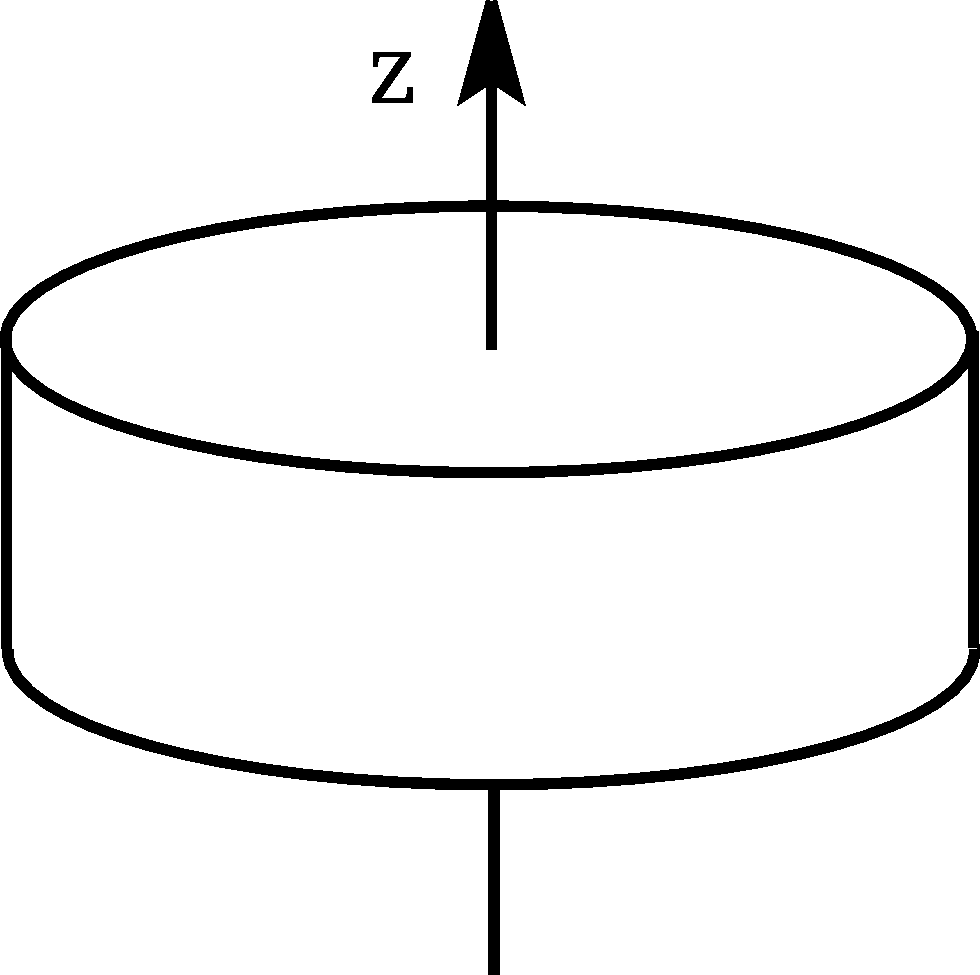
\includegraphics[scale=0.2]{Foucault.pdf}
\end{center}

\subsubsection*{Champ axial}

	Un champ magnétique uniforme $\vec{B}=B_{0}\vec{e_{z}}$ est appliqué.
	
	\begin{itemize}
	
		\item[$\diamondsuit$] En considérant la force de Lorentz qui s'exerce sur les électrons de conduction, analyser les effets de la rotation du cylindre pour justifier l'établissement d'un régime permanent. Existe t-il des courants des Foucault lorsque ce régime est établi ? 
		
	\item[$\diamondsuit$] En régime permanent, montrer à l'aide de la force de Laplace que l'effet du champ magnétique est équivalent à un champ électrique $\vec{E_m}$ dont on précisera l'expression. Quelle est alors la répartition des charges dans le cylindre ?
	
	\end{itemize}
	
	
\subsubsection*{Champ transverse}	
	
	On applique désormais un champ magnétique uniforme $\vec{B}=B_{0}\vec{e_{x}}$ transverse à l'axe de rotation.
	
\begin{itemize}
	
		\item[$\square$] Justifier l'existence de courants de Foucault dans ce cas en prévoyant leur allure. Quel est leur effet mécanique ?

\end{itemize}
		
Si le cylindre est très long, la densité de courant est de la forme $\vec{j}=j(r,\theta)\vec{e_{z}}$. On suppose de plus que les phénomènes électromagnétiques proches des extrémités supérieures et inférieures (les disques) sont négligeables par rapport à ceux ayant lieu le long du cylindre.

\begin{itemize}

		\item[$\square$] Quelle est la relation entre $j(r,\theta)$ et $j(r,\theta+\pi)$?
		
		\item[$\square$] En déduire le champ électrique $\vec{E}(r,t)$ à l'intérieur du cylindre.
		
		\item[$\square$] Exprimer alors l'expression de $\vec{j}(r,\theta)$ 
		
		\item[$\square$] Quelle est la puissance dissipée dans le cylindre ?
		
		\item[$\square$] Déterminer le moment des efforts de Laplace par rapport à l'axe de rotation.
		
\end{itemize}

\newpage

\section*{Canon électromagnétique}

On considère un circuit électrique équipé d'un générateur et de deux rails parallèles sur lesquels se trouve un barreau mobile, se déplaçant suivant $x$. L'inductance $L(x)$ et la résistance $R(x)$ dépendent alors de $x$. Le générateur impose un courant $I(t)$ à travers le circuit. 

\begin{figure}[h!]
\centering
		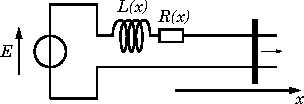
\includegraphics[scale=1]{induction1.pdf}
\end{figure}

\subsubsection*{Cas statique}

On suppose dans un premier temps que le mobile est fixé à $x=x_0$ et ne peut pas se mouvoir. 

\begin{itemize}

	\item[$\heartsuit$] Exprimer le flux magnétique à travers le circuit et en déduire la force électromotrice d'auto-induction.
	
	\item[$\heartsuit$] Lors de l'établissement du courant de 0 à $I(t)$, le générateur doit fournir une énergie magnétique $E_m$ en plus de l'énergie dissipée par effet Joule. Quelle est l'expression de $E_m$ ?

\end{itemize}

\subsubsection*{Cas mobile}

Le barreau est supposée désormais libre de ses mouvement selon l'axe $x$. 

\begin{itemize}

	\item[$\triangle$] Lorsqu'un courant électrique parcourt le circuit, le barreau se met en mouvement. Expliquer. Exprimer, à l'instant $t$, la puissance fournie par le générateur en sus de celle dissipée par effet Joule. 
	
	\item[$\triangle$] Une partie de cette puissance correspond à la variation de $E_m$, une autre correspond à la puissance mécanique $P_{méca}$ donnée au barreau. Donner l'expression de $P_{méca}$. Quelle force s'exerce sur le barreau ?

\end{itemize}

\subsubsection*{Étude du mouvement}

On suppose que le générateur est constitué d'une dynamo couplée à une bobine d'inductance $L_0$ et de résistance $R_0$. Tant que l'interrupteur $C$ est fermé, la dynamo impose un fort courant $I_0$ dans la bobine. A $t=0$, où l'on ouvre $C$, le courant s'écoule alors dans les rails et accélère le barreau. 

\begin{figure}[h!]
\centering
		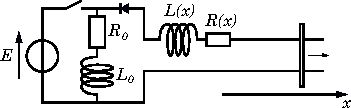
\includegraphics[scale=1]{induction2.pdf}
\end{figure}

On suppose par ailleurs que $L(x)=L'x$ et $R(x)=R'x$, où $L'$ et $R'$ sont respectivement l'inductance et la résistance linéique du barreau.

\begin{itemize}

	\item[$\diamondsuit$] Écrire la force électromotrice du circuit déformable, puis l'équation électrique du circuit. 
	
	\item[$\diamondsuit$] Ecrire l'équation du mouvmeent du barreau. On notera sa masse $M$. 
	
	\item[$\diamondsuit$] Quelles sont les conditions initiales ? Existe t-il des solutions stationnaires ?
	
	\item[$\diamondsuit$] On suppose que $L_0$ est très "grande". Justifier que $I(t)\simeq I_0$ et en déduire $\dot{x}(t)$ et $x(t)$.

\end{itemize}

Question supplémentaire : déterminer l'inductance et la résistance linéique dans le cas de deux rails cylindriques de rayon $a$, distants de $b$ et de conductivité $\gamma$.

\end{document}
